\subsection{NAT Traversal}
\label{sec:p2p:nat-traversal}

It is expected that many, if not most, of the end users in the HOPR network operate behind one or more network address translation mechanisms (NATs). This can include an opaque address mapping of the ISP if it uses \href{https://en.wikipedia.org/wiki/Carrier-grade_NAT}{carrier-grade NAT}, the local router bridging between local network and the internet, as well as containerized environments which add an additional address mapping to translate between host and guest machines.

Due to this, it is for most nodes unlikely to establish a direct connection to other nodes. Nevertheless, it is in most cases possible to determine a way how to connect directly by exchanging signalling information using a different means of communication. Within the HOPR network, this is achieved by relay nodes that act as rendezvous points and allow nodes to negotiate how to connect directly. In case, there is no direct possible, e.g. because of bidirectional NATs or restrictive firewalls, the relayed connection acts as a fallback.

Hence, when connecting to another node, the initiator runs through three phases: first it attempts to connect directly using published IP address and port and if not successful, it tries to connect to one of the relay nodes and thereby establishes the fallback connection. Meanwhile the nodes exchange first messages, both of the gather information how to traverse their NAT mechanism and transparently replace the connection by a direct WebRTC connection.

\begin{figure}[H]
    \centering
    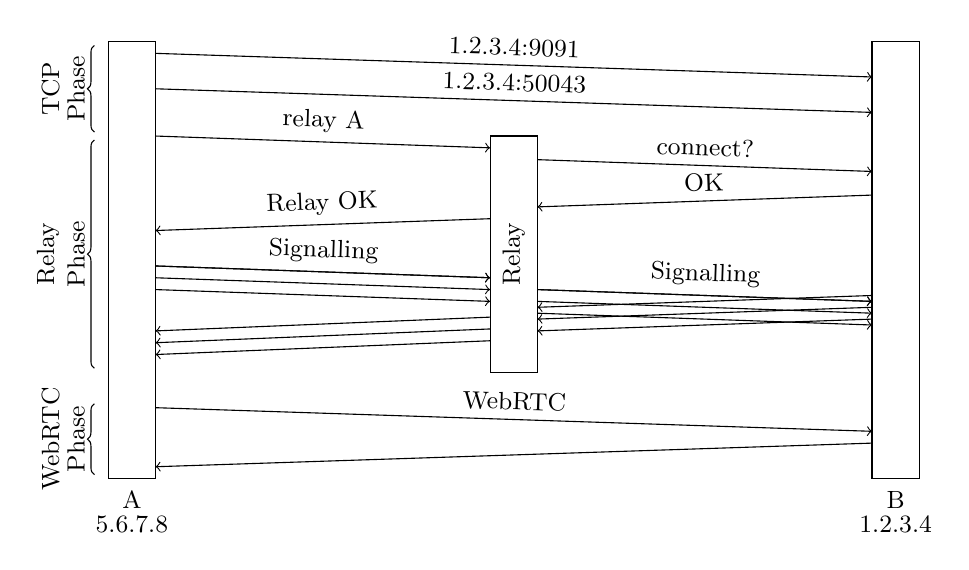
\begin{tikzpicture}
        \def\nodeHeight{5.55}
        \def\nodeWidth{0.6}
        \def\nodeOffset{4.25}
        \def\relayPhaseOffset{1.2}
        \def\webRTCOffset{4.65}
        \def\padding{0.05}

        % Nodes A and B
        \foreach \offset\name\address in{0/A/5.6.7.8,2*\nodeWidth+2*\nodeOffset/B/1.2.3.4} {
                \draw[shift={(\offset,0)}] (0,0) rectangle node[below=80pt] {\small{\shortstack{\name\\\address}}}(\nodeWidth,-\nodeHeight) ;
            }

        % Relay
        \draw (\nodeWidth+\nodeOffset,-\relayPhaseOffset) rectangle (\nodeWidth+\nodeOffset+\nodeWidth,-4.2) node[midway] {\rotatebox{90}{\small{Relay}}};

        % TCP phase
        \draw[->,shift={(0,-0.15)}] (\nodeWidth,0) -- (2*\nodeWidth+2*\nodeOffset,-0.3) node[midway,above,sloped] {\small{1.2.3.4:9091}};
        \draw[->,shift={(0,-0.6)}] (\nodeWidth,0) -- (2*\nodeWidth+2*\nodeOffset,-0.3) node[midway,above,sloped] {\small{1.2.3.4:50043}};

        \draw[decoration={brace,raise=5pt,mirror},decorate] (0,-\padding) -- node[left=5pt] {\rotatebox{90}{\small{\shortstack{TCP\\Phase}}}} (0,-\relayPhaseOffset+\padding);

        % Relay phase
        \begin{scope}[shift={(0,-\relayPhaseOffset)}]
            \draw[->] (\nodeWidth,0) -- (\nodeWidth+\nodeOffset,-0.15) node[midway,above,sloped] {
                \small{relay A}};

            \draw[->,shift={(1*\nodeWidth+\nodeOffset,-0.3)}] (\nodeWidth,0) -- (\nodeWidth+\nodeOffset,-0.15) node[midway,above,sloped] {\small{connect?}};

            \draw[->,shift={(1*\nodeWidth+\nodeOffset,-0.75)}] (\nodeWidth+\nodeOffset,0) -- (\nodeWidth,-0.15) node[midway,above,sloped] {\small{OK}};

            \draw[->] (\nodeOffset+\nodeWidth,-1.05) -- (\nodeWidth,-1.2) node[midway,above,sloped] {\small{Relay OK}};

            \foreach \i in{0,1,2} {
                    \begin{scope}[shift={(0,-1.65)}]
                        \ifnum\i=0
                            \draw[->] (\nodeWidth,0) -- (\nodeOffset+\nodeWidth,-0.15) node[midway,above,sloped] {\small{Signalling}};
                            \draw[->] (2*\nodeWidth+\nodeOffset,-0.3) -- (2*\nodeOffset+2*\nodeWidth,-0.45) node[midway,above,sloped] {\small{Signalling}};
                        \fi
                        \ifnum\i<3
                            \draw[->] (\nodeWidth,-\i*0.15) -- (\nodeOffset+\nodeWidth,-0.15-\i*0.15);
                            \draw[->] (2*\nodeWidth+\nodeOffset,-0.3-\i*0.15) -- (2*\nodeOffset+2*\nodeWidth,-0.45-\i*0.15);
                            \draw[->] (2*\nodeWidth+2*\nodeOffset,-0.375-\i*0.15) -- (\nodeOffset+2*\nodeWidth,-0.525-\i*0.15);
                            \draw[->] (\nodeWidth+\nodeOffset,-0.65-\i*0.15) -- (\nodeWidth,-0.825-\i*0.15);
                        \fi
                    \end{scope}
                }

            \draw[decoration={brace,raise=5pt,mirror},decorate] (0,-\padding) -- node[left=5pt] {\rotatebox{90}{\small{\shortstack{Relay\\Phase}}}} (0,-4.2+\relayPhaseOffset+\padding);
        \end{scope}

        % WebRTC phase
        \begin{scope}[shift={(0,-\webRTCOffset)}]
            \draw[->] (\nodeWidth,0) -- (2*\nodeWidth+2*\nodeOffset,-0.3) node[midway,above,sloped] {\small{WebRTC}};
            \draw[->] (2*\nodeWidth+2*\nodeOffset,-0.45) -- (\nodeWidth,-0.75);
            \draw[decoration={brace,raise=5pt,mirror},decorate] (0,\padding) -- node[left=5pt] {\rotatebox{90}{\small{\shortstack{WebRTC\\Phase}}}} (0,-0.9+\padding);
        \end{scope}
    \end{tikzpicture}
\end{figure}
